\mbox{$\displaystyle $\,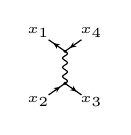
\begin{tikzpicture}[x=0.340cm, y=0.340cm, line width=0.420pt, baseline={([yshift=-0.6ex]0,0)}]
  \draw plot[smooth, tension=0.7] coordinates {(0.000,0.600) (0.065,0.557) (0.093,0.514) (0.065,0.471) (0.000,0.429) (-0.065,0.386) (-0.093,0.343) (-0.065,0.300) (0.000,0.257) (0.065,0.214) (0.093,0.171) (0.065,0.129) (0.000,0.086) (-0.065,0.043) (-0.093,0.000) (-0.065,-0.043) (0.000,-0.086) (0.065,-0.129) (0.093,-0.171) (0.065,-0.214) (0.000,-0.257) (-0.065,-0.300) (-0.093,-0.343) (-0.065,-0.386) (0.000,-0.429) (0.065,-0.471) (0.093,-0.514) (0.065,-0.557) (0.000,-0.600)};
  \draw (0.000,0.600) -- (-0.614,1.030);
  \fill (-0.436,0.905) -- (-0.299,0.685) -- (-0.304,0.813) -- (-0.182,0.852) -- cycle;
  \draw (0.000,-0.600) -- (-0.614,-1.030);
  \fill (-0.179,-0.725) -- (-0.433,-0.778) -- (-0.311,-0.818) -- (-0.316,-0.946) -- cycle;
  \draw (0.000,-0.600) -- (0.614,-1.030);
  \fill (0.436,-0.905) -- (0.299,-0.685) -- (0.304,-0.813) -- (0.182,-0.852) -- cycle;
  \draw (0.000,0.600) -- (0.614,1.030);
  \fill (0.179,0.725) -- (0.433,0.778) -- (0.311,0.818) -- (0.316,0.946) -- cycle;
  \fill (0.000,0.600) circle (0.064);
  \fill (0.000,-0.600) circle (0.064);
  \node[font=\tiny, inner sep=0pt, anchor=325] at (-0.688,1.082) {$x_{1}$};
  \node[font=\tiny, inner sep=0pt, anchor=35] at (-0.688,-1.082) {$x_{2}$};
  \node[font=\tiny, inner sep=0pt, anchor=145] at (0.688,-1.082) {$x_{3}$};
  \node[font=\tiny, inner sep=0pt, anchor=215] at (0.688,1.082) {$x_{4}$};
\end{tikzpicture}}
\diagramgap
\mbox{$\displaystyle -\,$\,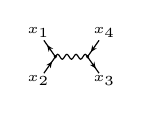
\begin{tikzpicture}[x=0.340cm, y=0.340cm, line width=0.420pt, baseline={([yshift=-0.6ex]0,0)}]
  \draw plot[smooth, tension=0.7] coordinates {(-0.600,0.000) (-0.557,0.065) (-0.514,0.093) (-0.471,0.065) (-0.429,0.000) (-0.386,-0.065) (-0.343,-0.093) (-0.300,-0.065) (-0.257,0.000) (-0.214,0.065) (-0.171,0.093) (-0.129,0.065) (-0.086,0.000) (-0.043,-0.065) (0.000,-0.093) (0.043,-0.065) (0.086,0.000) (0.129,0.065) (0.171,0.093) (0.214,0.065) (0.257,0.000) (0.300,-0.065) (0.343,-0.093) (0.386,-0.065) (0.429,0.000) (0.471,0.065) (0.514,0.093) (0.557,0.065) (0.600,0.000)};
  \draw (-0.600,0.000) -- (-1.030,0.614);
  \fill (-0.905,0.436) -- (-0.852,0.182) -- (-0.813,0.304) -- (-0.685,0.299) -- cycle;
  \draw (-0.600,0.000) -- (-1.030,-0.614);
  \fill (-0.725,-0.179) -- (-0.946,-0.316) -- (-0.818,-0.311) -- (-0.778,-0.433) -- cycle;
  \draw (0.600,0.000) -- (1.030,-0.614);
  \fill (0.905,-0.436) -- (0.852,-0.182) -- (0.813,-0.304) -- (0.685,-0.299) -- cycle;
  \draw (0.600,0.000) -- (1.030,0.614);
  \fill (0.725,0.179) -- (0.946,0.316) -- (0.818,0.311) -- (0.778,0.433) -- cycle;
  \fill (-0.600,0.000) circle (0.064);
  \fill (0.600,0.000) circle (0.064);
  \node[font=\tiny, inner sep=0pt, anchor=305] at (-1.082,0.688) {$x_{1}$};
  \node[font=\tiny, inner sep=0pt, anchor=55] at (-1.082,-0.688) {$x_{2}$};
  \node[font=\tiny, inner sep=0pt, anchor=125] at (1.082,-0.688) {$x_{3}$};
  \node[font=\tiny, inner sep=0pt, anchor=235] at (1.082,0.688) {$x_{4}$};
\end{tikzpicture}}
